\documentclass[border=10pt]{standalone}
\usepackage[svgnames]{xcolor}
\usepackage{amsmath}
\usepackage{pgfplots}
\pgfplotsset{compat=newest}
\usepackage[sfdefault]{FiraSans}
\usepackage{FiraMono}
\renewcommand*\familydefault{\sfdefault}
\begin{document}
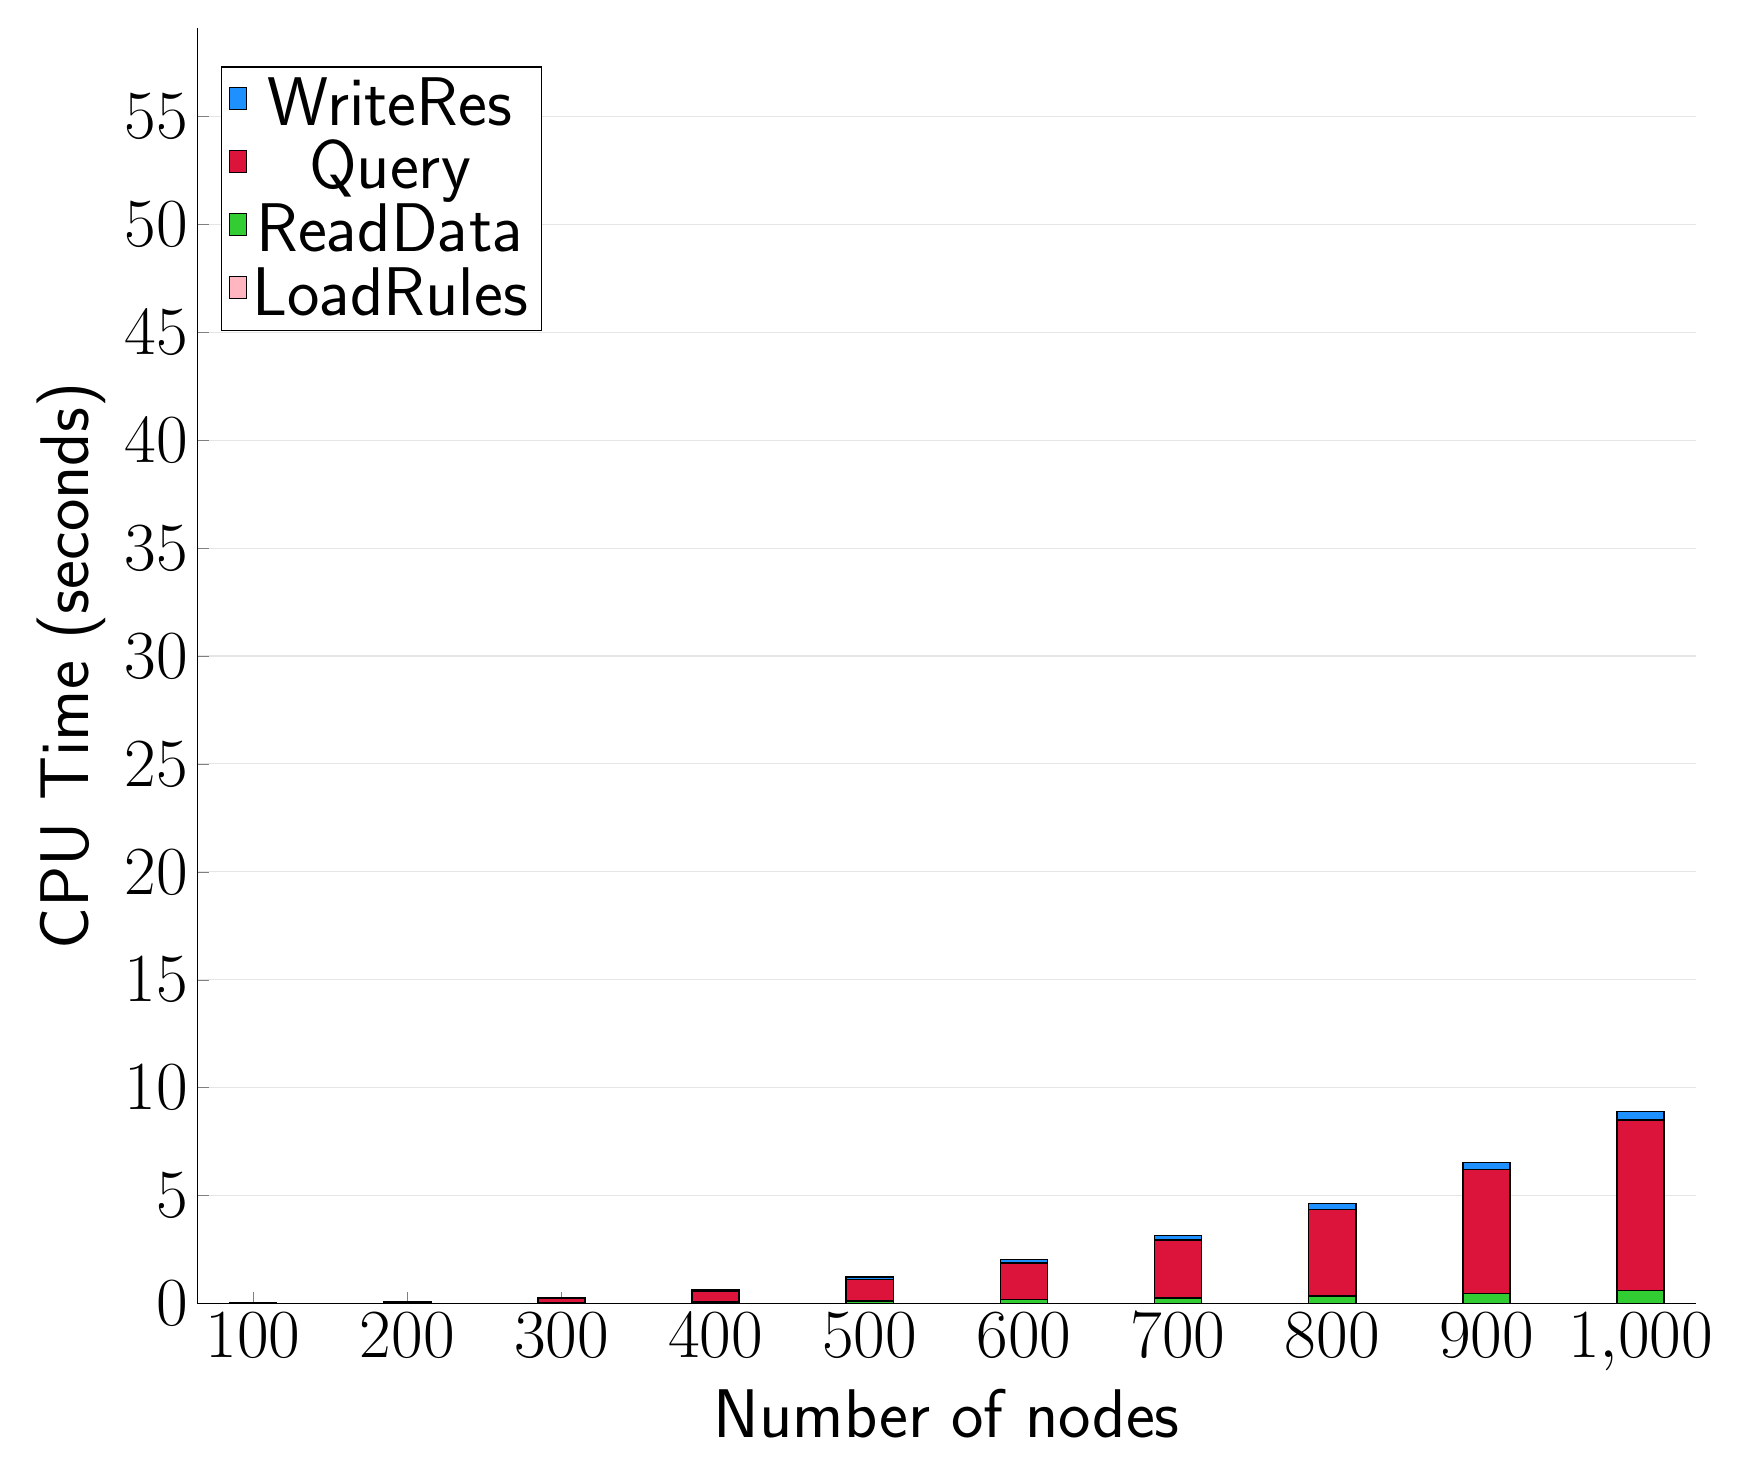
\begin{tikzpicture}
\begin{axis}[
   ybar stacked,
   width=1.7\textwidth,
   bar width=0.6cm,
   ymajorgrids, tick align=inside,
   major grid style={draw=gray!20},
   xtick=data,
   ymin=0, ymax=59.082040000000006,
   axis x line*=bottom,
   axis y line*=left,
   enlarge x limits=0.04,
   legend style={
       at={(0.23, 0.97)},
       anchor=north east,
       legend columns=1,
       font=\Huge,
   },
   ylabel={CPU Time (seconds)},
   xlabel={Number of nodes},
   label style={font=\Huge},
   tick label style={font=\Huge},
]
\addlegendimage{fill=DodgerBlue, draw=black, line width=0.2pt}
\addlegendentry{WriteRes}
\addlegendimage{fill=Crimson, draw=black, line width=0.2pt}
\addlegendentry{Query}
\addlegendimage{fill=LimeGreen, draw=black, line width=0.2pt}
\addlegendentry{ReadData}
\addlegendimage{fill=LightPink, draw=black, line width=0.2pt}
\addlegendentry{LoadRules}
\addplot +[fill=LightPink, draw=black, line width=0.55pt] coordinates {
(100, 0.0005519999999999998)
(200, 0.000553)
(300, 0.000551)
(400, 0.0005531999999999998)
(500, 0.0005528000000000002)
(600, 0.0005619999999999998)
(700, 0.0005554000000000003)
(800, 0.0005547999999999997)
(900, 0.0005510000000000004)
(1000, 0.0005592)
};
\addplot +[fill=LimeGreen, draw=black, line width=0.55pt] coordinates {
(100, 0.0040447999999999994)
(200, 0.0170934)
(300, 0.040194999999999995)
(400, 0.07461960000000001)
(500, 0.1219422)
(600, 0.1840564)
(700, 0.26083680000000004)
(800, 0.3577032)
(900, 0.46859779999999995)
(1000, 0.6110244)
};
\addplot +[fill=Crimson, draw=black, line width=0.55pt] coordinates {
(100, 0.0081346)
(200, 0.0646892)
(300, 0.2161836)
(400, 0.5093488)
(500, 1.0045911999999997)
(600, 1.7000406)
(700, 2.6842528)
(800, 4.010453)
(900, 5.7381466)
(1000, 7.883575800000001)
};
\addplot +[fill=DodgerBlue, draw=black, line width=0.55pt] coordinates {
(100, 0.0040352)
(200, 0.016613)
(300, 0.03637000000000001)
(400, 0.06663279999999998)
(500, 0.10192140000000002)
(600, 0.15044999999999997)
(700, 0.20661520000000005)
(800, 0.25999580000000017)
(900, 0.3189255999999997)
(1000, 0.3932047999999998)
};
\end{axis}
\end{tikzpicture}

\end{document}
